\subsection{Introducci�n}
El objetivo de esta parte es familiarizarse con el simulador \textit{simusched}, el cual sirve para ver el comportamiento de distintos lotes
de procesos bajo distintas pol�ticas de scheduling. Adicionalmente se puede especificar la cantidad de cores a disposici�n de los procesos, y
los costos de ciertas acciones como hacer un cambio de contexto, o cambiar un proceso para que se ejecute en otro core.
\subsection{Ejercicio 1}
El objetivo de este ejercicio es implementar una tarea de tipo \textbf{TaskConsola}, la cual debe simular ser una tarea interactiva.
Para esto, la tarea realiza $n$ llamadas bloqueantes, cada una con una duraci�n al azar entre \textit{bmin} y \textit{bmax}, ambos 
especificados por par�metro. La implementaci�n de esta funci�n es bastante directa, y b�sicamente consiste en inicializar el generador de 
n�meros aleatorios con el par�metro \textit{time(NULL)}, es decir, con la fecha actual al momento de ejecutarse la funci�n. Luego, se realizan
$n$ llamadas bloqueantes con una duraci�n al azar entre \textit{bmin} y \textit{bmax}, utilizando la funci�n \texttt{uso\_IO}. Para m�s detalles, 
consultar la implementaci�n en el archivo \textit{tasks.cpp}.
\subsection{Ejercicio 2}
El objetivo de este ejercicio es ejecutar un lote de tareas, una intensiva en CPU y las otras 2 de tipo interactivo (\textbf{TaskConsola}), con
la pol�tica de scheduling \textbf{FCFS}, y observar y graficar los resultados, variando la cantidad de cores.


El lote de tarea que utilizamos es el \textit{lote1.tsk}. A continuaci�n se pueden ver los gr�ficos:

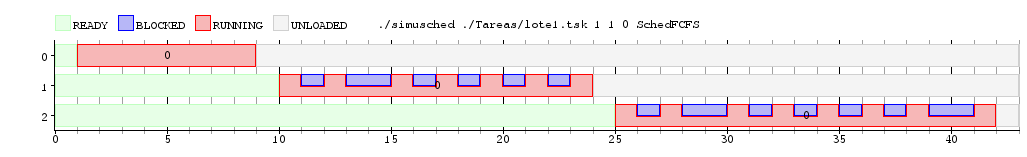
\includegraphics[width=1\textwidth]{./Graficos/ej2_1.png}
\begin{center}
 \textit{1 core}.
\end{center}

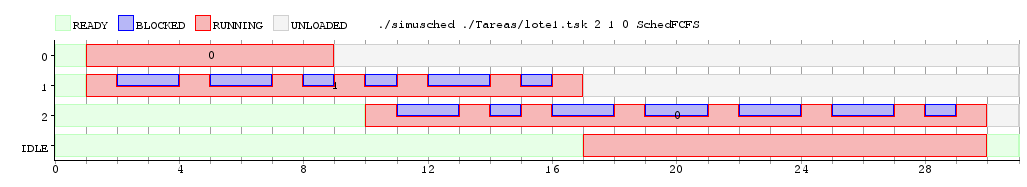
\includegraphics[width=1\textwidth]{./Graficos/ej2_2.png}
\begin{center}
 \textit{2 cores}.
\end{center}

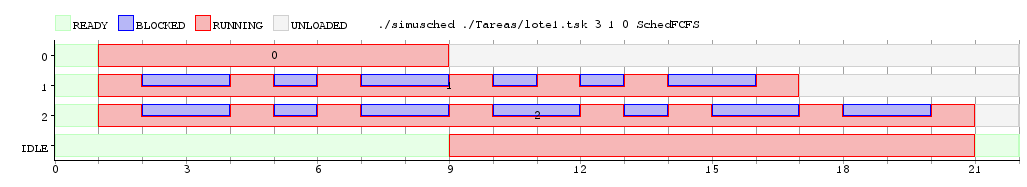
\includegraphics[width=1\textwidth]{./Graficos/ej2_3.png}
\begin{center}
 \textit{3 core}.
\end{center}